\documentclass{article}

\usepackage{url}
\usepackage{hyperref}
\usepackage{natbib}
\usepackage{graphicx}
%\usepackage{aas_macros}
%\usepackage{multirow}

\def\mnras{MNRAS}


\begin{document}
\section{The MultiNest Algorithm}
The MultiNest algorithm is a Bayesian inference tool for parameter space exploration and model selection that has come to widespread use in Astrophysics and Cosmology over the past years. 

It builds upon the nested sampling technique producing the Bayesian evidence by integrating the likelihood associated with a given set of parameters over the multidimensional parameter space, and creates samples of the posterior distribution as a by-product.

The novel way in which MultiNest represents the sampled volume by an optimized set of ellipsoids makes it especially powerful for exploring multi-modal posteriors or posteriors with curving degeneracies in high dimensions.

Our implementation follows the full description of the algorithm in \cite{2009MNRAS.398.1601F}.
\section{Performance}
put comparison tables and colorful pictures here
\subsection{Lighthouse example}

\subsection{Toy model 1: ``egg-box''}
Although our implementation is currently lacking one major feature from  \cite{2009MNRAS.398.1601F}, mode identification (described in section 5.6), we can use the test cases presented there to gauge our code's performance.

The first toy model is called the egg-box likelihood. It is designed to show MultiNest's performance in highly multimodal problems. Instead of deriving the likelihood function from observed data and a realistic model, it is given analytically:
\[L(\theta_1,\theta_2) = \mathrm{exp}
\left[\left\{2+\cos\left(\frac{\theta_1}{2}\right)+\cos\left(\frac{\theta_2}{2}\right)\right\}^5\right]\]
The likelihood function and its sampling returned by a run of our code with 2000 points is shown in figure~\ref{eggbox}.

\begin{figure}\label{eggbox}
\includegraphics[width=0.5\textwidth]{figures/eggbox_analytic.pdf}
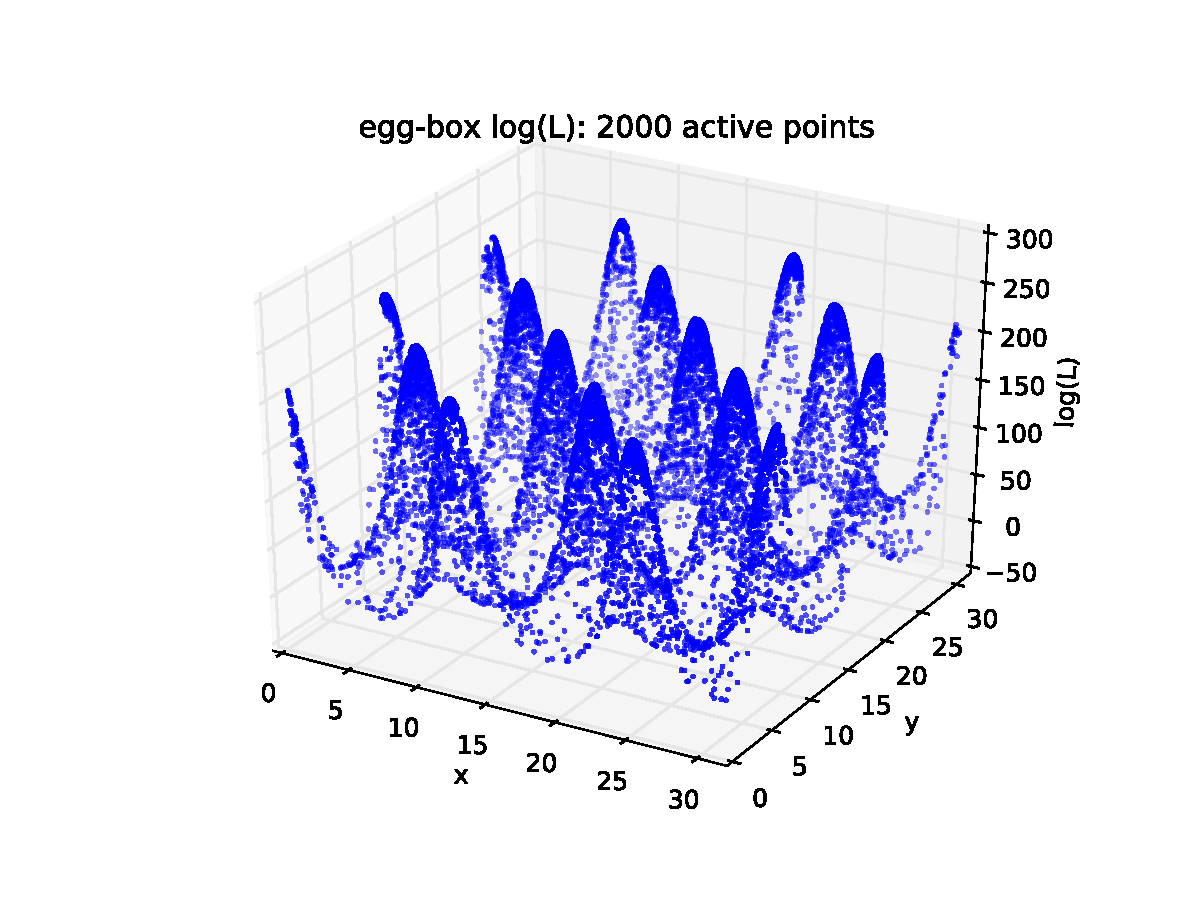
\includegraphics[width=0.5\textwidth]{figures/eggbox.pdf}
\caption{Analytical and sampled likelihood function of the eggbox toy model}
\end{figure}

Given the analytical likelihood, the total log-evidence can be numerically integrated to 235.88. Our algorithm gives a result of $235.57\pm 0.06$ which is too low. Presumably, a bug either in the uniform sampling or in the final integration after convergenge limits our accuracy. This deviation will be investigated further.

\subsection{Toy model 2: ``gaussian shells''}
The second toy model in \cite{2009MNRAS.398.1601F} tests MultiNest's performance with curving degeneracies and high dimensionalities. The analytic likelihood function is given by
\[L(\theta) = \mathrm{circ}(\theta;c_1,r_1,w_1)+\mathrm{circ}(\theta;c_2,r_2,w_2)\]
where
\[ \mathrm{circ}(\theta;c,r,w) = \frac{1}{\sqrt{2\pi w^2}}\mathrm{exp}\left[-\frac{(|\theta - c|-r)^2}{2w^2}\right]\]
The two dimensional appearance of this likelihood function is shown in figure~\ref{gauss-shell}.

\begin{figure}\label{gauss-shell}
\includegraphics[width=0.5\textwidth]{figures/gauss_shells_analytic.pdf}
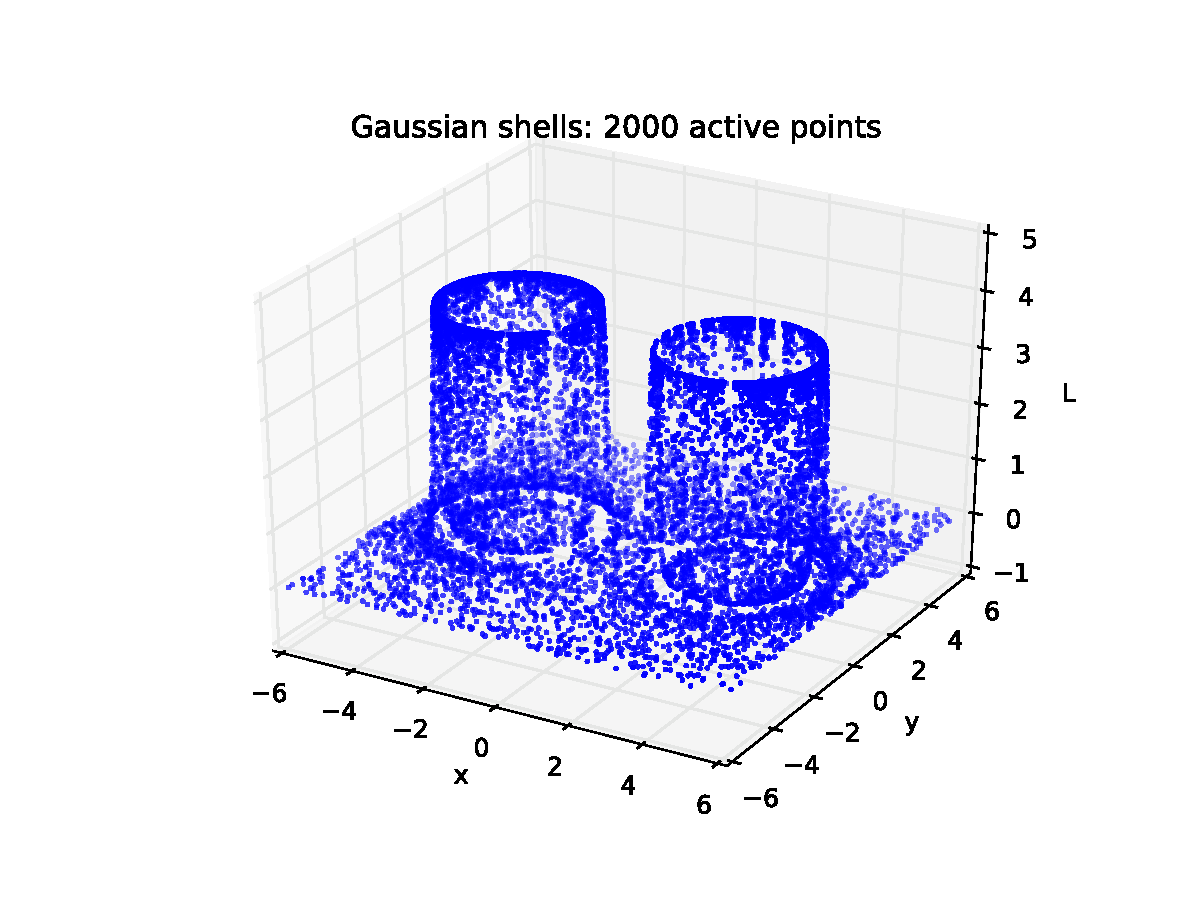
\includegraphics[width=0.5\textwidth]{figures/gauss_shells.pdf}
\caption{Analytical and sampled likelihood function of the gaussian-shells toy model}
\end{figure}

The total log-likelihood evaluates to $-1.75$, while our algorithm returns $-1.41\pm 0.03$  with 2000 points.

\subsection{Profiled run}
\section{User Instructions}
this is where the README-equivalent can go
\bibliographystyle{myplainnat}
\bibliography{writeup}

\end{document}
